\documentclass{article}
\usepackage[utf8]{inputenc}
\usepackage[danish]{babel}
\usepackage{amsmath}
\usepackage{ulem}
\usepackage{palatino}
\usepackage{graphicx}
\usepackage{verbatim}
\linespread{1.05}
\title{Advanced Algorithms - Assignment 2}
\author{Ronni Elken Lindsgaard\and
Troels Henriksen\and
Jacob Wejendorp}
\begin{document}
\maketitle
\section{Traveling Couple Problem}
For $d=0$ TCP is identical to TSP for all input graphs. And for $d > 0$
there will always be graphs where the minimum vertice distance is
greater than $d$, in which case the problem is again equivalent to TSP, which
is known NP-complete. Therefore we cannot say whether TCP is solvable in
polynomial time.

\subsection{Data structure}

A candidate solution is a path through the graph, which we represent
as an ordered sequence of vertices.  Implemented in a programming
language it could be either a linked list or an indexed array.  We
assume that the path need not return to its origin.

\subsection{Initial candidate solution}

$V$ is intialised to the empty set. We then start by choosing an
arbitrary vertice $v$ and add it to the set $V$.  Afterwards we take
another arbitrary vertice not in the set $V$ and not within the
distance $d$ from a node in $V$.  Repeat this until no such nodes are
left.

\subsection{Mutation operators}

We make use of the following two mutation operators:

\begin{itemize}
\item We take two arbitrary edges $(u_1,v_1)$ and $(u_2,v_2)$ and
  replace them with $(u_1,u_2)$ and $(v_1,v_2)$. The switch of
  directions is propagated through the subgraph that connects $v_1$
  and $u_2$, in the form of reversing the list.
\item We take a vertice $v$ from the set $V$ and look at all vertices
  within range $d$ of $v$. We then choose an arbitrary vertice $u$
  from this set and check if it is possible to replace $u$ with $v$
  and still have all nodes covered.
\end{itemize}

\subsection{Implementation of hill-climbing}

For one hundred runs, the average cost (path length) is
$26.4827292786505$, and the minimum is $24.4202464069$.

\section{Tabu-search}
We have implemented a feature-based Tabu-search, that uses the altered nodes in the tweak procedure,
as its tabu-elements, making tabu any tweak that includes changing such a vertice.
This requires all tweaks to keep a list of nodes it alters and return it to the algorithm.
The algorithm then keeps this list, being subject to the length contraint $l$, and discards all tweaks that return
a node currently in the tabu-list.

In essence a direct implementation of "Algorithm 15 Feature-based Tabu Search" from Essentials of Metaheuristics, p 25.\\

The results using Tabu-search are significantly better than Hill-climbing, which is primarily caused by
tabus more explorative nature, which means it will look at a larger sample, and is more likely to find
any solution. This, however is not unlike a simple steepest-ascent algorithm, in which the algorithm
also considers a larger neighborhood than hillclimbing. This shows as the result-difference between a
tabu-search and steepest-ascent in our case shows little difference in results.


\section{Best solution}
We have found a tour of length $23.1677$, using feature-based Tabu-search with a $n=20,l=30$ distribution.\\
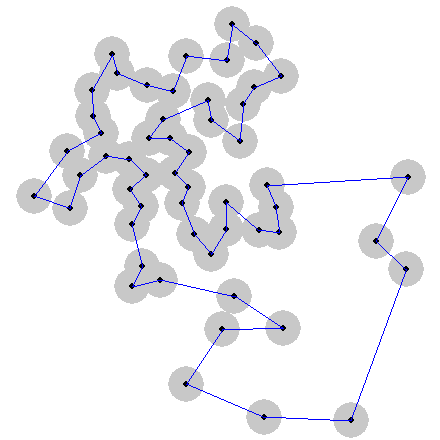
\includegraphics[width=100mm]{solution-2316.png}

\appendix

\section{Hill-Climbing Implementation}

\verbatiminput{src/florence.py}


\section{Tabu-search implementation}

\verbatiminput{pyMetaheuristics/Algorithms/TabuSearch.py}

\end{document}
